\documentclass[a4paper,10pt,landscape,twocolumn]{article}

%Math
\usepackage{amsmath}
\usepackage{amsfonts}
\usepackage{amssymb}
\usepackage{amsthm}
\usepackage{ulem}
%\usepackage{stmaryrd} %f\UTF{00FC}r Blitz!

%PageStyle
\usepackage[ngerman]{babel} % deutsche Silbentrennung
\usepackage[utf8]{inputenc} 
\usepackage{fancyhdr, graphicx}
\usepackage[scaled=0.92]{helvet}
\usepackage{enumitem}
\usepackage{parskip}
\usepackage[a4paper,top=2cm]{geometry}
\setlength{\textwidth}{25cm}
\setlength{\oddsidemargin}{-0.5cm}


%My Commands
\newcommand{\RN}{\mathbb{R}} %Real Number
\newcommand{\NN}{\mathbb{N}} %Natural Number
\newcommand{\QN}{\mathbb{Q}} %Rational Number
\newcommand{\ZN}{\mathbb{Z}} %ganze Zahlen
\newcommand{\CN}{\mathbb{C}}
\newcommand{\Teilt}{\mid} %\mid
\newcommand{\Teiltn}{\nmid} %kein teiler
\newcommand{\Potp}{\mathcal{P}} %Potenzmenge
\newcommand{\Pota}{\mathcal{A}}
\newcommand{\Potr}{\mathcal{R}}
\newcommand{\Potn}{\mathcal{N}}
\newcommand{\Bold}[1]{\textbf{#1}} %Boldface
\newcommand{\Kursiv}[1]{\textit{#1}} %Italic
\newcommand{\T}[1]{\text{#1}} %Textmode
\newcommand{\Nicht}[1]{\T{\sout{$ #1 $}}} %Streicht Shit durch
\newcommand{\lra}{\leftrightarrow} %Arrows
\newcommand{\ra}{\rightarrow}
\newcommand{\la}{\leftarrow}
\newcommand{\lral}{\longleftrightarrow}
\newcommand{\ral}{\longrightarrow}
\newcommand{\lal}{\longleftarrow}
\newcommand{\Lra}{\Leftrightarrow}
\newcommand{\Ra}{\Rightarrow}
\newcommand{\La}{\Leftarrow}
\newcommand{\Lral}{\Longleftrightarrow}
\newcommand{\Ral}{\Longrightarrow}
\newcommand{\Lal}{\Longleftarrow}
\newcommand{\Vektor}[1]{\vec{#1}}
\newcommand{\Brace}[1]{\left( #1 \right)} %()
\newcommand{\Bracel}[1]{\left\lbrace #1 \right.} %(
\newcommand{\Bracer}[1]{\right. #1 \right\rbrace} %)
\newcommand{\Brack}[1]{\left\lbrace #1 \right\rbrace} %{}
\newcommand{\Brackl}[1]{\left\lbrace #1 \right.} %{
\newcommand{\Brackr}[1]{\right. #1 \right\rbrace} %}
\newcommand{\Result}[1]{\underline{\underline{#1}}} %Doppelt unterstrichen
\newcommand{\Abs}[1]{\left\mid #1 \right\mid} %Absolutbetrag
\newcommand{\Norm}[1]{\Abs{\Abs{ #1 }}} %Norm
\newcommand{\Arrays}[1]{\left(\begin{array}{c}#1\end{array}\right)} %Array mit einer Kolonne ()
\newcommand{\Array}[2]{\left(\begin{array}{#1}#2\end{array}\right)} %Array mit n Kolonnen ()
\newcommand{\Bracka}[2]{\left\lbrace\begin{array}{#1}#2\end{array}\right\rbrace} %Array mit {}
\newcommand{\Brackal}[2]{\left\lbrace\begin{array}{#1} #2 \end{array}\right.} %Array mit {
\newcommand{\Brackar}[2]{\left.\begin{array}{#1} #2 \end{array}\right\rbrace} %Array mit }
\newcommand{\Sumone}[2]{\sum_{#2=1}^{#1}} %Summe von 1
\newcommand{\Sumz}[2]{\sum_{#2=0}^{#1}} %Summe von 0
\newcommand{\Sum}[2]{\sum_{#2}^{#1}} %Allgemeine Summe
\newcommand{\Oneover}[1]{\frac{1}{#1}} %1 über igendwas
\newcommand{\Tablewt}[3]{\begin{table*}[h]\caption{#1} \begin{tabular}{#2}{#3}\end{tabular}\end{table*}} %Table mit Titel
\newcommand{\Oben}[2]{\overset{#1}{#2}} %etwas über etwas anderem
\newcommand{\Unten}[2]{\underset{#1}{#2}} %etwas unter etwas anderem
\newcommand{\Bildcap}[2]{\begin{figure}[htb]\centering\includegraphics[width=0.2\textwidth]{#1} \caption{#2}\end{figure}} %Bild mit beschriftung
\newcommand{\Bildjpeg}[1]{\includegraphics[width=0.2\textwidth]{#1.jpeg}} %Bilder jpeg!!
\newcommand{\Bildjpg}[1]{\includegraphics[width=0.2\textwidth]{#1.jpg}} %Bilder jpg!!
\newcommand{\Bild}[1]{\includegraphics[width=0.4\textwidth]{#1}} %Bilder jpg!!
%Beispiel für lstlisting \lstinputlisting[label=Aufgabe 4a,caption=Aufgabe 4a]{4a.java}

% Code listenings
\usepackage{color}
\usepackage{xcolor}
\usepackage{listings}
\usepackage{caption}
\DeclareCaptionFont{white}{\color{white}}
\DeclareCaptionFormat{listing}{\colorbox{gray}{\parbox{\textwidth}{#1#2#3}}}
\captionsetup[lstlisting]{format=listing,labelfont=white,textfont=white}
\lstdefinestyle{JavaStyle}{
 language=Java,
 basicstyle=\footnotesize\ttfamily, % Standardschrift
 numbers=left,               % Ort der Zeilennummern
 numberstyle=\tiny,          % Stil der Zeilennummern
 stepnumber=5,              % Abstand zwischen den Zeilennummern
 numbersep=5pt,              % Abstand der Nummern zum Text
 tabsize=2,                  % Groesse von Tabs
 extendedchars=true,         %
 breaklines=true,            % Zeilen werden Umgebrochen
 frame=b,         
 %commentstyle=\itshape\color{LightLime}, Was isch das? O_o
 %keywordstyle=\bfseries\color{DarkPurple}, und das O_o
 basicstyle=\footnotesize\ttfamily,
 stringstyle=\color[RGB]{42,0,255}\ttfamily, % Farbe der String
 keywordstyle=\color[RGB]{127,0,85}\ttfamily, % Farbe der Keywords
 commentstyle=\color[RGB]{63,127,95}\ttfamily, % Farbe des Kommentars
 showspaces=false,           % Leerzeichen anzeigen ?
 showtabs=false,             % Tabs anzeigen ?
 xleftmargin=17pt,
 framexleftmargin=17pt,
 framexrightmargin=5pt,
 framexbottommargin=4pt,
 showstringspaces=false      % Leerzeichen in Strings anzeigen ?        
}

%Config
\renewcommand{\headrulewidth}{0pt}
\setlength{\headheight}{15.2pt}

%Metadata
\title{
	%\vspace{5cm}
	Eti Zusammenfassung
}
\author{Rebeca Stuber, Jasmin Lienhard \& Fabio Oesch}
\date{5. Semester (HS 2014)}


% hier beginnt das Dokument
\begin{document}

% Titelbild
\maketitle
\thispagestyle{fancy}

\pagebreak

% Inhaltsverzeichnis
\pagenumbering{Roman}
\tableofcontents	  	


\pagebreak
\setcounter{page}{1}
\pagenumbering{arabic}

\section{Endliche Automaten}
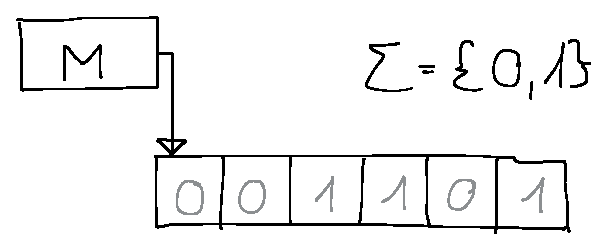
\includegraphics[width=0.3\textwidth,height=4cm,keepaspectratio]{Bild1.eps}\\
\Bold{Def:} Ein endlicher Automat (deterministisch) ist ein 5-Tupel $A=(Q,\Sigma,\delta,q_0,F)$
\begin{description}
 \item [$Q$] Menge der Zust\"ande
 \item [$\Sigma$] Alphabet
 \item [$\delta$] $Q\times\Sigma\to Q$ \"Ubergangsfunktion
 \item [$q_0$] Startzustand
 \item [$F\subset Q$] akzeptierende Zust\"ande
\end{description}
\Bold{Bsp:} Sei $A=(Q,\Sigma,\delta,q_0,F)$\\
mit $Q=\{q_0,q_1,q_2\}$, $\Sigma=\{0,1\}$, $F=\{q_1\}$\\
\begin{tabular}{c|c|c}
 $\delta$&0&1\\\hline
 $q_0$&$q_0$&$q_1$\\
 $q_1$&$q_2$&$q_2$\\
 $q_2$&$q_1$&$q_2$\\
\end{tabular}\\
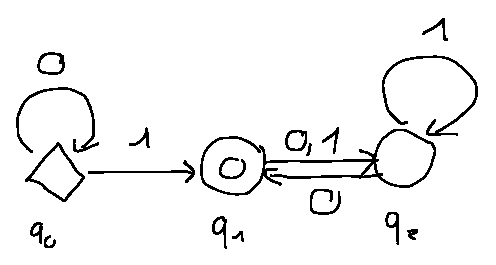
\includegraphics[width=0.3\textwidth,height=4cm,keepaspectratio]{Bild3.eps}\\
Antwortfunktion von $A$\\
$r_A:\Sigma^*\to Q$\\
\Bold{Bsp:} $r_A(0,0,1,0)=q_2 \notin F\Rightarrow0010\notin L(A)$\\
$L(A)=\{\omega\in\Sigma^*\mid r_A(\omega)\in F\}$
\subsubsection{Notation}
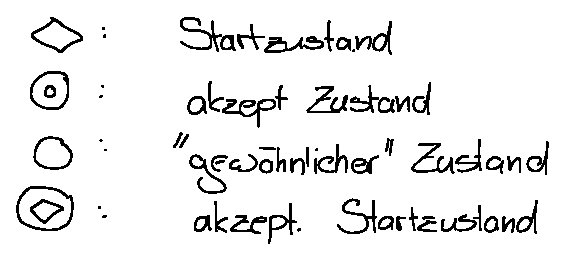
\includegraphics[width=0.3\textwidth,height=4cm,keepaspectratio]{Bild2.eps}
\subsection{Satz 1}
\Bold{Vor:} $A\in DFA$\\
\Bold{Beh:} $L(A)$ ist regul\"ar\\
\Bold{Beweisidee:}\\
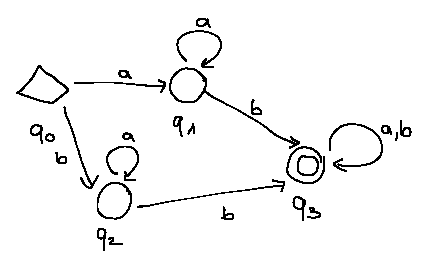
\includegraphics[width=0.3\textwidth,height=4cm,keepaspectratio]{Bild4.eps}\\
$\Sigma=\{0,1\}$\\
$G=(N,T,Q,S)$ regul\"ar mit $L(G)=L(A)$\\
$T=\Sigma=\{a,b\}$\\
$N=\{S=Sq_0,Sq_1,Sq_2,Sq_3\}$\\
$R=\{Sq_0\to aSq_1\mid bSq_2,Sq1\to aSq1\mid bSq3,Sq2\to aSq2\mid bSq3,Sq3\to aSq3\mid bSq3\mid a\mid b\}$
\begin{enumerate}
 \item Zuordnung: Zustand $\mapsto$ Nichtterminalsymbol
 \item Jedem Pfeil im Diagramm ordnen wir eine oder zwei Regeln zu
 \begin{enumerate}
  \item $q_i\Oben{a}{\to}q_j$ mit $a_j\notin F$\\
  $\Rightarrow Sq_i\to a Sq_j$
  \item $q_i\Oben{a}{\to}a_j$ mit $q_j\in F$\\
  $Sq_i\to a Sq_j$\\
  $Sq_i\to a$
 \end{enumerate}
\end{enumerate}
\Bold{Bsp:}\\ 
a) Das Wort aab akzeptieren. $q_0\to q_1\to q_1\to q_3$\\
b) Das Wort aab generieren. $Sq_0\Rightarrow aSq_1\Rightarrow aaSq_1\Rightarrow aab$

\subsection{Nicht-deterministische, endliche Automaten (NFA)}
\Bold{Bsp:}\\
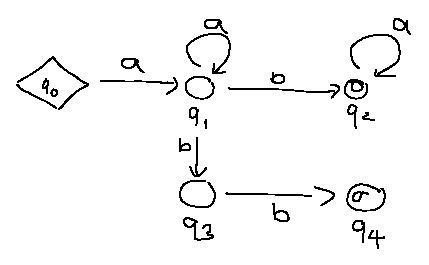
\includegraphics[width=0.3\textwidth,height=4cm,keepaspectratio]{Bild5.eps}\\
$baa\notin L(A)$, $aab\in L(A)$\\
\begin{tabular}{l|c|c}
 $\delta$&$a$&$b$\\\hline
 $q_0$&$\{q_1\}$&$\emptyset$\\
 $q_1$&$\{q_1\}$&$\{q_2,q_3\}$\\
 $q_2$&$\{q_2\}$&$\emptyset$\\
 $q_3$&$\emptyset$&$\{q_4\}$\\
 $q_4$&$\emptyset$&$\emptyset$
\end{tabular}
\Bold{Satz:} \Bold{Vor.} $A\in NFA$ \Bold{Beh.} $\exists B\in DFA:L(A)=L(B)$\\
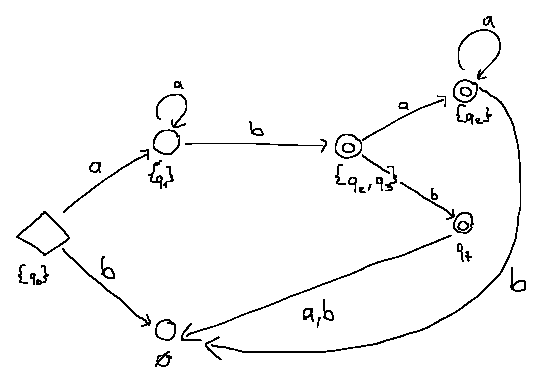
\includegraphics[width=0.3\textwidth,height=4cm,keepaspectratio]{Bild6.eps}\\
\begin{tabular}{l|c|c}
 $\overline{\delta}$&$a$&$b$\\\hline
 $\{q_0\}$&$\{q_1\}$&$\emptyset$\\
 $\{q_1\}$&$\{q_1\}$&$\{q_2,q_3\}$\\
 $\{q_2,q_3\}$&$\{q_2\}$&$\{q_4\}$\\
 $\{q_2\}$&$\{q_2\}$&$\emptyset$\\
 $\{q_4\}$&$\emptyset$&$\emptyset$\\
 $\emptyset$&$\emptyset$&$\emptyset$\\
\end{tabular}\\
$\overline{F}=\{a_2,a_3\},\{a_2\},\{a_4\}$\\
\Bold{Satz:} \Bold{Vor.} $L\subset \Sigma^*$ regul\"ar, \Bold{Beh.} $\exists A\in NFA:L(A)=L$\\
\Bold{Beweis} regul\"ar $\Rightarrow\exists$ regul\"are Grammatik $G=(N,T,R,S)$\\
mit $N=\{S,A,B,\dots\}$, $T=\Sigma$, $R=\{\dots A\to aB$, $A\to a\dots\}$
\begin{enumerate}
 \item Jedem Nichtterminalsymbol ordnen wir einen Zustand zu. z.B. $A\mapsto q_A$
 \item Jeder Regel vom Typ $A\to aB$ ordnen wir einen Pfeil im Diagramm zu: $q_A\Oben{a}{\to}q_B$
 \item Wir f\"ugen einen \Bold{neuen} akzeptierenden Zustand $E$ zu $Q$ hinzu und f\"ur jede Regel $A\to b$ ein Pfeil $q_A\Oben{b}{\to}E$\\
 $Q=\{q_S,q_A,q_B,\dots,E\}$
\end{enumerate}
\subsection{DFA}
\Bold{Bsp:} $\Sigma=\{a,b\}$, $G=(N,T,R,S)$\\
mit $N=\{S,A\}$, $T=\Sigma$, $R=\{S\to aA,S\to a,A\to bA, A\to b\}$\\
$\Bold{A}:=(Q,\Sigma,\delta,q_S,F)$\\
$Q=\{q_S,q_A,E\}$\\
$F=\{E\}$\\
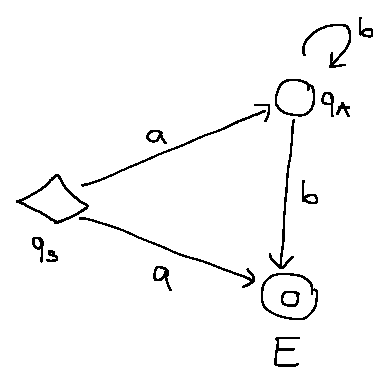
\includegraphics[width=0.3\textwidth,height=4cm,keepaspectratio]{Bild7.eps}\\
\begin{tabular}{l|c|c}
 $\overline{\delta}$&$a$&$b$\\\hline
 $\{q_S\}$&$\{q_A,E\}$&$\emptyset$\\
 $\{q_A,E\}$&$\emptyset$&$\{q_A,E\}$\\
 $\emptyset$&$\emptyset$&$\emptyset$\\
\end{tabular}\\
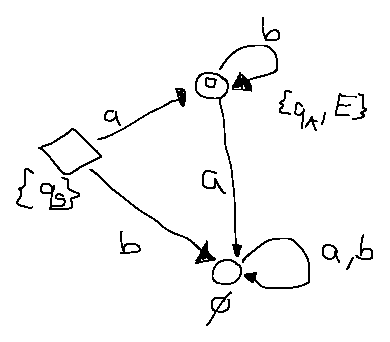
\includegraphics[width=0.3\textwidth,height=4cm,keepaspectratio]{Bild8.eps}\\
\Bold{Def.} Zwei endliche Automaten $A$ und $B$ heisen \Bold{\"aquivalent}: $\Leftrightarrow L(A)=L(B)$
\subsection{NFA$/\varepsilon$}
\Bold{Bsp:} $(^*)$ $A=(Q,\Sigma,\delta,q_0,F)$\\
$\Sigma=\{a,b\}$, $Q=\{q_0,q_1,q_2,q_3\}$, $F=\{q_2\}$\\
\begin{tabular}{l|c|c|c}
 ${\delta}$&$a$&$b$&$\varepsilon$\\\hline
 $q_0$&$q_1$&$q_2$&$\emptyset$\\
 $q_1$&$\emptyset$&$\emptyset$&$q_2$\\
 $q_2$&$\emptyset$&$q_1$&$q_3$\\
 $q_3$&$q_2$&$q_3$&$\emptyset$
\end{tabular}\\
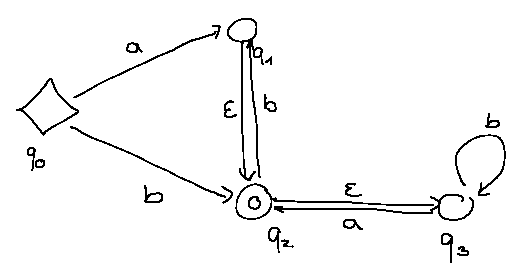
\includegraphics[width=0.3\textwidth,height=4cm,keepaspectratio]{Bild9.eps}\\
\subsubsection{$\varepsilon$-H\"ullen der Zust\"ande}
$[q]_\varepsilon^*:=\{r\in Q\mid q\Oben{\varepsilon^*}{\to}r\}$\\
\Bold{Bsp anhand Bild 9}\\
$[q_0]_\varepsilon^*=\{q_0\}$, $[q_1]_\varepsilon^*=\{q_1,q_2,q_3\}$, $[q_2]_\varepsilon^*=\{q_2,q_3\}$, $[q_3]_\varepsilon^*=\{q_3\}$\\
\Bold{NFA}\\
$B=(\overline{Q},\Sigma,\overline{\delta},\overline{q_0},\overline{F})$\\
\begin{equation} 
 \overline{\delta}(q,a)=\bigcup_{r\in[q]_\varepsilon^*}\delta(r,a)
\end{equation}

\begin{tabular}{c|c|c}
 $\overline{\delta}$&$a$&$b$\\\hline
 $q_0$&$\{q_1\}$&$\{q_2\}$\\
 $q_1$&$\{q_2\}$&$\{q_1,q_3\}$\\
 $q_2$&$\{q_2\}$&$\{q_1,q_3\}$\\
 $q_3$&$\{q_2\}$&$\{q_3\}$
\end{tabular}\\
$\overline{F}=\{q\in Q\mid [q]_\varepsilon^*\cap F\neq \emptyset\}$
\subsection{Eigenschaften regul\"arer Sprachen}
Sei $\Sigma$ ein Alphabet\\
$C\subset P(\Sigma*)$ Menge von Sprachen\\
\Bold{Frage:} F\"uhren Operationen auf den Elementen von $C$ aus $C$ heraus?\\
\Bold{Bsp:} von Operationen\\
$\overline{L}:=\Sigma*\backslash L$\\
$L_1\cup L_2$\\
$L_1 \cap L_2$\\
$L_1\cdot L_2=\{\omega_1\omega_2|\omega_1\in L_1,\omega_2\in L_2\}$\\
\Bold{Bsp:} $L_1 =\{0,1\}$ ,$L_2 =\{\varepsilon,1\}$ $\Rightarrow L_1\cdot L_2 = \{0\varepsilon, 1\varepsilon,01,11\}$
\Bold{Notation:}
$L^0:=\{\varepsilon\}$\\
$L^1:= L$\\
$L^2:= L\cdot L$ (Konkatenation)\\ 
$L^3:= L\cdot L^2 = L^2\cdot L$
\subsubsection{*- oder Kleene-Operation}
$L^*:=L^0\cup L^1\cup L^2\cup L^3\cup\dots$\\
\Bold{Bsp:} $\Sigma=\{0,1\}$, $\Sigma^*=\{\varepsilon\}\cup\{0,1\}\cup\{00,01,10,11\}\cup\dots$
\Bold{Notation:} $Reg_\Sigma:=$ Menge der regul\"aren Sprachen \"uber $\Sigma$.\\
\Bold{Satz:} \Bold{Vor.} $L_1,L_2\in Reg_\Sigma$\\
\Bold{Beh.} $\overline{L_1},L_1\cup L_2,L_1\cap L_2,L_1\cdot L_2,L_1^*\in Reg_\Sigma$\\[\baselineskip]
\Bold{Bew.}
\begin{enumerate}
 \item $I_1\in Reg_\Sigma\Ra\exists A=(Q,\Sigma,\delta,q_0,F)\in DFA$ mit $L(A)=L$\\
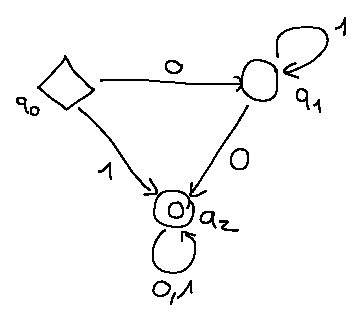
\includegraphics[width=0.3\textwidth,height=4cm,keepaspectratio]{Bild10.eps}\\
 $L(A)=\{1w,01^*0\omega|\omega\in\Sigma^*\}$\\
 $\overline{L(A)}=\{01^*,\varepsilon\}$\\
 $\overline{A}:=(Q,\Sigma,\delta,q_0,\overline{F}:=Q\backslash F)$\\
 $L(\overline{A})=I$\\
 \Bold{Achtung:} Gilt nur f\"ur DFA's!
 \Bold{Bsp:}\\
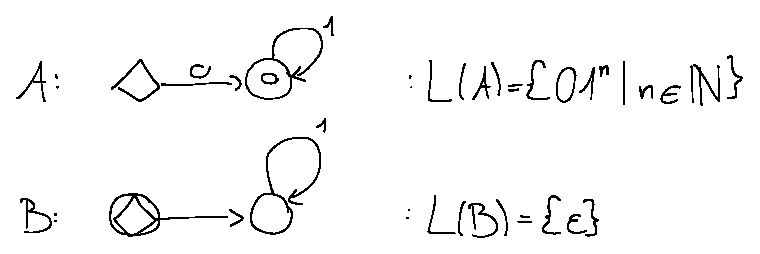
\includegraphics[width=0.3\textwidth,height=4cm,keepaspectratio]{Bild12.eps}\\
 \item $L_1\cup L_2\in Reg_\Sigma$\\
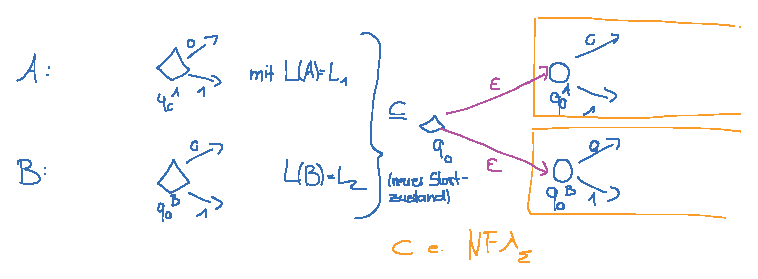
\includegraphics[width=0.3\textwidth,height=4cm,keepaspectratio]{Bild11.eps}\\
 $L(C)=L_1\cup L_2$
 \item $L_1\cap L_2\in Reg_\Sigma$\\
 \Bold{1. Beweis} De Morgan: $L_1\cap L_2 = \overline{\overline{L_1}\cup\overline{L_2}}$\\
 \Bold{Bsp:}\\
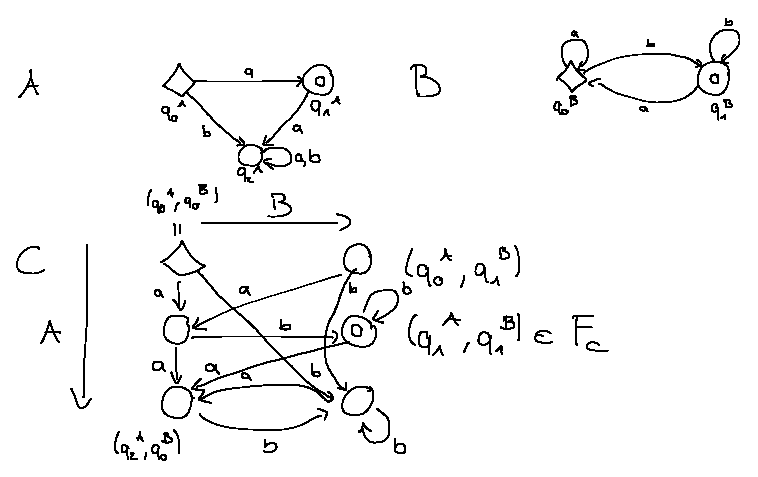
\includegraphics[width=0.3\textwidth,height=4cm,keepaspectratio]{Bild13.eps}\\
 \item $L_1\cdot L_2\in Reg_\Sigma$\\
 $L_1=\{01^+\}$\\
 $L_2=\{\varepsilon,01,11,101\}$\\
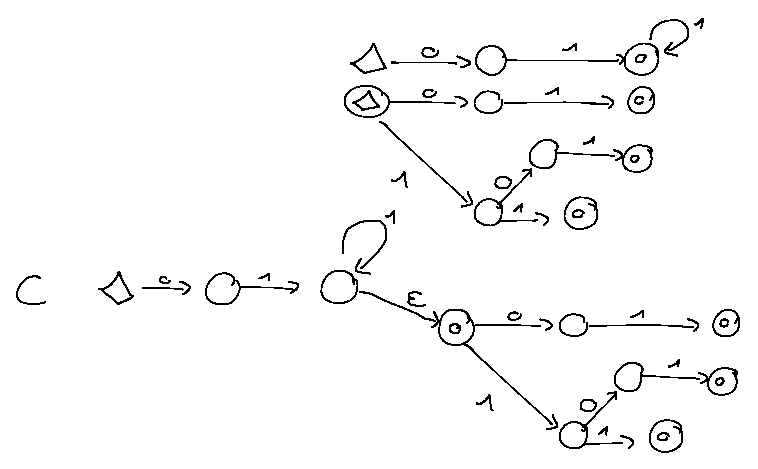
\includegraphics[width=0.3\textwidth,height=4cm,keepaspectratio]{Bild15.eps}\\
 \item $L_1^*\in Reg_\Sigma$\\
 $L=\{01^*001^*\}$\\
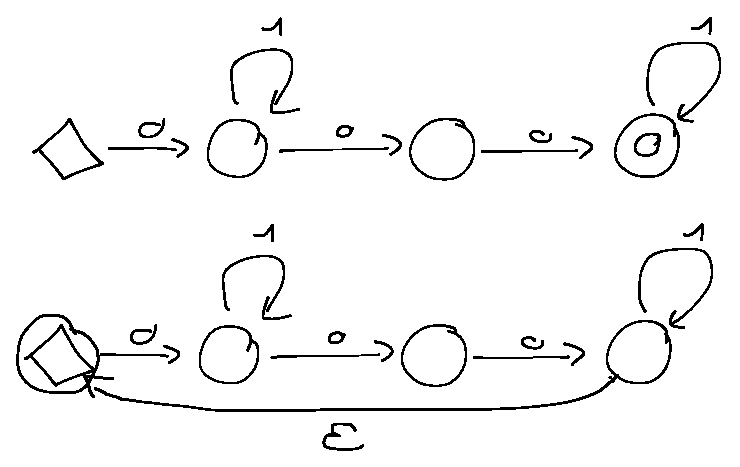
\includegraphics[width=0.3\textwidth,height=4cm,keepaspectratio]{Bild16.eps}\\
\end{enumerate}
\subsection{Das Pumping-Lemma und der Satz von Myhill-Nerode}
\Bold{Frage:} Wie zeigen wir, dass eine Sprache $L\notin Reg_\Sigma$?\\
\Bold{Gegeben:} $L\in Reg_\Sigma\Ra\exists A=(Q,\Sigma,\delta,q_0,F)\in DFA$\\
$n:=\mid Q\mid$ (Anzahl der Zust\"ande)
\subsubsection{Pumping Lemma}
\Bold{Vor.} $L\in Reg_\Sigma$\\
\Bold{Beh.} $\exists n \in \NN^*: \forall\omega\in L,\mid\omega\mid\geq n\exists x,y,z\in\Sigma^*$\\
$x$ ist Weg vom Anfangszustand zum wiederholenden Zustand, $y$ ist der Loop (vom wiederholenden zum wiederholenden Zustand), $z$ der Weg vom wiederholenden Zustand zum akzeptierenden Zustand
\begin{enumerate}
 \item $\omega=xyz$
 \item $\mid y\mid \geq 1$
 \item $\mid xy\mid\leq n$
 \item $\forall i\in \NN: xy^iz\in L$
\end{enumerate}
\Bold{Bsp:}
\begin{enumerate}
 \item $\Sigma=\{0,1\}$, $L=\{0^k1^k\mid k\in \NN^*\}$\\
 $G=(N,T,R,S)$, $N=\{S\}$, $T=\{0,1\}$, $R=\{S\to 01,S\to0S1\}$ (kontextfrei) $\} = L(G)=L$\\
 \Bold{Annahme $L$ ist regul\"ar}\\
 $\forall n\in\NN^*$: W\"ahlen wir ein Wort $\omega_n\in L$ mit $\mid\omega_n\mid\geq n$.\\
 $\omega_n=0^n1^n=$
 \begin{tabular}{|l|l|}
  $0\dots\dots0$&$1\dots\dots1$\\\hline
  \multicolumn{2}{|l|}{$x\mid y\mid z\Ra$ 3. Bedingung: $y=0\dots0\geq1$}
 \end{tabular}
  ($\mid\omega_n\mid=2n$)\\
  Bedingung 4: $xyyz\in L$ geht nicht, da mindestens eine weitere 0 hinzugef\"ugt wird.\\
  $\Ra $ Die Sprache ist kontextfrei denn $xz\notin L$
\end{enumerate}
\Bold{Bsp.} $G_{arith}^n=(N,T,R,<arithm Ausdruecke>)$ // $<AA>$\\
$N=\{<AA>,<Vor>\}$, $T=\{(,),+,-,x_1,x_2,\dots,x_n\}$\\
$R=\{<AA>\to<Var>$, $<Var>\to x_1$, $<Var>\to x_2$, $\dots$, $<Var>\to x_n$, $<AA>\to(<AA>+<AA>)$, $<AA>\to(<AA>\cdot <AA>)\}$\\
\Bold{Augfaben:}
\begin{enumerate}
 \item Gegeben f\"ur Bsp f\"ur W\"orter aus $L(G^n_{arith})$\\
 $x_1,x_2,x_n,(x_1+x_2)$
 \item Welcher Klasse geh\"ort $G^n_{arith}$ an.\\
 kontextfrei
 \item In welchek Klasse liegt $L(G^n_{arith})$\\
 Es wird angenommen, dass die Sprache nicht regul\"ar ist, da man Z\"ahlen muss, wieviele Klammern ge\"offnet worden sind.\\
 \Bold{Annahme:} $L(G^n_{arith})\in Reg$\\
 $n\in \NN^*$ $\omega_n$\\
 $\omega_n = \underbrace{(((((\dots(}_nx_1+x_2)\dots)$\\
 Da $\mid xy\mid\leq n$ und $y\neq\varepsilon\Ra y=(^n\mid n\in\NN$\\
 $\omega_n=xyz$, $\tilde{\omega}=xyyz\notin L(G^n_{arith})$
\end{enumerate}
Falls man Z\"ahlen muss ist die Sprache mit grosser Wahrscheinlichkeit keine regul\"are Sprache. Z\"ahlen bedeutet zum Beispiel, dass bei $0^n1^n$ man die Nullen z\"ahlen muss da es genau gleich viele Einsen haben muss.\\
\Bold{Bsp.} $\Sigma=\{0,1\}$\\
$L=\{\omega\in\Sigma^*\mid\omega\T{ endet auf }00\}$\\
Erste Frage: Was sind die \"Aquivalezklassen? $R_L=[\varepsilon],[0],[00]$, $\Sigma^*=[\varepsilon]\cup[0]\cup[00]$\\
$A=(Q,\Sigma,\delta,q_0,F)$, $Q=\{[\varepsilon],[0],[00]\}$, $q_0:=[\varepsilon]$, $F:=\{[00]\}$, $\delta([\omega],a):=[\omega a]$\\
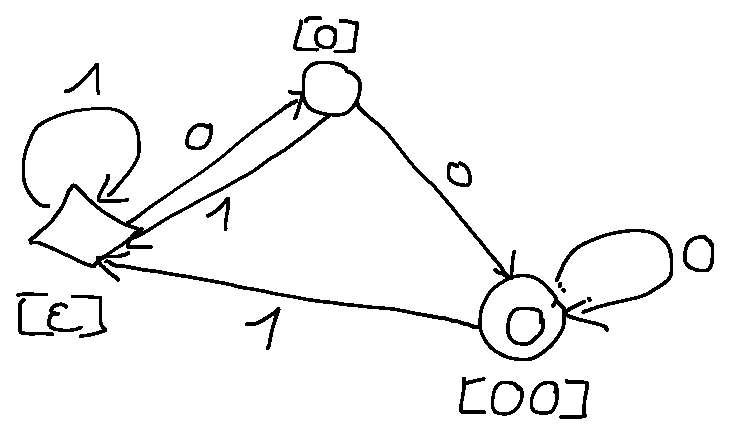
\includegraphics[width=0.3\textwidth,height=4cm,keepaspectratio]{Bild17.eps}\\
\subsubsection{Satz von Myhill-Nerode}
Anzahl der \"Aquivalezklassen wird definiert durch $ind(R):=|\{[x]\mid x\in M\}|$\\
\Bold{Satz 2.33 (Myhill-Nerode)} Es sei $L\subset \Sigma^*$ eine Sprache. $L$ ist genau dann regul\"ar, wenn $ind(R_L)<\infty$
\subsection{Minimierung endlicher Automaten (gilt nur f\"ur DFA)}
\Bold{Problem:} Gegeben: $A=(Q,\Sigma,\delta,q_0,F)$ mit $L(A)=L$\\
Gesucht: Minimaler DFA, der $L$ akzeptiert.\\
\Bold{Notation:} Sei $q\in Q$\\
$L(A,q):=\{\omega\in\Sigma^*\mid r_A(q,\omega)\in F\}$\\
\Bold{Bsp.} $L(A,q_0)=L(A)$\\
Wir f\"uhren auf $Q$ eine Relation $RL_A$ ein:\\
Seien $q_l,q_j\in Q$\\
$(q_l,q_j)\in RL_A:\Lra L(A,q_i)=L(A,q_j)$\\
\Bold{Bem.} $RL_A$ ist eine \"Aquivalenzrelation
\subsubsection{Minimaler Automat}
\begin{enumerate}
 \item Elimination von aus $q_0$ nicht erreichbaren Zust\"anden
 \item Bestimmen der \"Aquivalezklassen von $RL_A$
 \item $A_{Min}=(\bar{Q},\Sigma,\bar{\delta},\bar{q_0},\bar{F})$\\
 mit $\bar{Q}:=\{[q]\mid q\in Q\}$, $\bar{q_0}:=[q_0]$, $\bar{F}:=\{[q]\mid q\in F\}$, $\bar{\delta}:=[\delta(q,a)]$
\end{enumerate}
\subsubsection{Algorithmus zur Bestimmung der \"Aquivalezklassen von $RL_A$}
\begin{enumerate}
 \item $\forall q_i,q_j\in Q$ mit $q_i\in Q\backslash F$ und $a_j\in F\Ra [q_i]\neq [q_j]$\\
 \Bold{Beweis.} $\varepsilon\notin L(A,q_i)$ und $\varepsilon\in L(A,q_j)$
 \item Sei $[q_i]\neq[q_j]$ und $\tilde{q_k},\tilde{q_e}\in Q$\\
 $\exists a\in\Sigma:\Brackal{l}{\Brackar{l}{\delta(\tilde{q_k},a)=q_i\\\delta(\tilde{q_e},a)=q_j}}\Ra[\tilde{q_k}]\neq[\tilde{q_e}]$\\
 $L(A,q_i)\neq L(A,q_j)\Ra L(A,\tilde{q_k}\neq L(A,\tilde{q_e})$
\end{enumerate}
$A\in DFA$\\
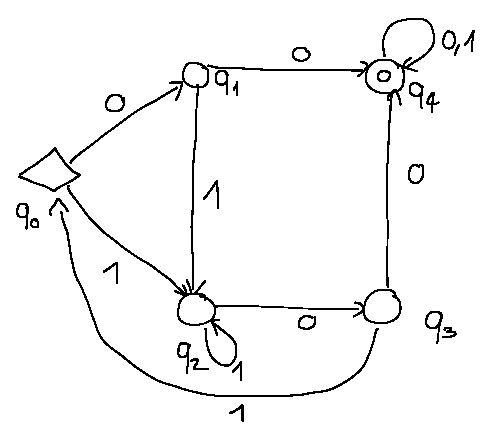
\includegraphics[width=0.3\textwidth,height=4cm,keepaspectratio]{Bild18.eps}\\
\begin{tabular}{c|c|c|c|c|}
 \hline $q_1$&$\star_1^0$&-&-&-\\\hline
 $q_2$&&$\star_1^0$&-&-\\\hline
 $q_3$&$\star_1^0$&&$\star_1^0$&-\\\hline
 $q_4$&$\star_0$&$\star_0$&$\star_0$&$\star_0$\\\hline
 &$q_0$&$q_1$&$q_2$&$q_3$
\end{tabular}\\
$RL_A=\{[q_0],[q_1],\Nicht{[q_2]},\Nicht{[q_3]},[q_4]\}$\\
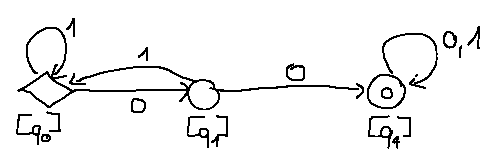
\includegraphics[width=0.3\textwidth,height=4cm,keepaspectratio]{Bild19.eps}\\
\section{Weiteres}
\subsection{Chomsky-Hierarchie}
\begin{tabular}{|c|c|c|}\hline
 Klasse&Bezeichnung&Bedingung\\\hline\hline
 0&allgemein&keine\\\hline
 1&kontextsensitiv&$u=\omega_1A\omega_2,v=\omega_1\omega\omega_2$ mit $A\in N$,\\
 &&$\omega_1,\omega_2\in(N\cup T)^*$, $\omega\in(N\cup T)^+$.\\\hline
 2&kontextfrei&$u\in N$, $v\in(N\cup T)^+$\\\hline
 3&regul\"ar&$u\in N$, $v=a$ oder $v=aA$ (oder $v=Aa$)\\
 &&mit $a\in T$, $A\in N$\\\hline
\end{tabular}\\
\Bold{Bemerkung 1.8} Die Regeln der Klassen 1 , 2 und 3 sind nicht verkürzend $|u|\leq |v|$. Deshalb können Grammatiken der Klassen 1 , 2 und 3 , wie sie oben beschrieben sind, keine Sprachen erzeugen, die das leere Wort enthalten. Um auch solche Sprachen beschreiben zu können, lassen wir zu, dass diese Grammatiken die Regel $S\to\varepsilon$ enthalten dürfen. In diesem Fall darf aber das Startsymbol S nur auf der linken Seite von Regeln erscheinen.\\
\Bold{Bemerkung 1.9} Eine Grammatik mit Regeln der Form $v = aA$ heisst rechts-linear, eine mit Regeln der Form $v = Aa$ heisst links-linear. Die Menge der rechts- und links-linearen Grammatiken bildet die Klasse der regulären Grammatiken. Eine Grammatik mit Regeln der Form $v = aA$ und der Form $v = Aa$ heisst linear und ist nicht regulär.\\
\Bold{Bemerkung 1.10} Es gilt Klasse 3 $\subset$ Klasse 2 $\subset$ Klasse 1 $\subset$ Klasse 0.\\
\Bold{Beispiel 1.11} Wenn eine Sprache durch eine kontextsensitive und eine reguläre Grammatik erzeugt werden kann, dann ist die Klasse der Sprache regulär.\\
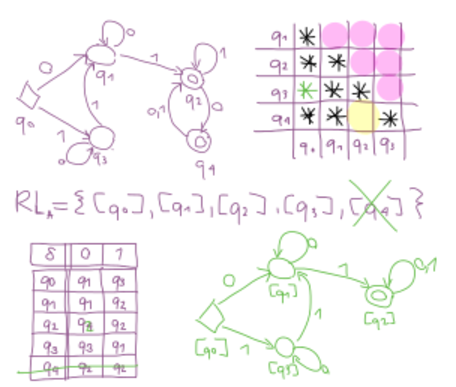
\includegraphics[width=0.4\textwidth,keepaspectratio]{Bild2Zufa.pdf}\\
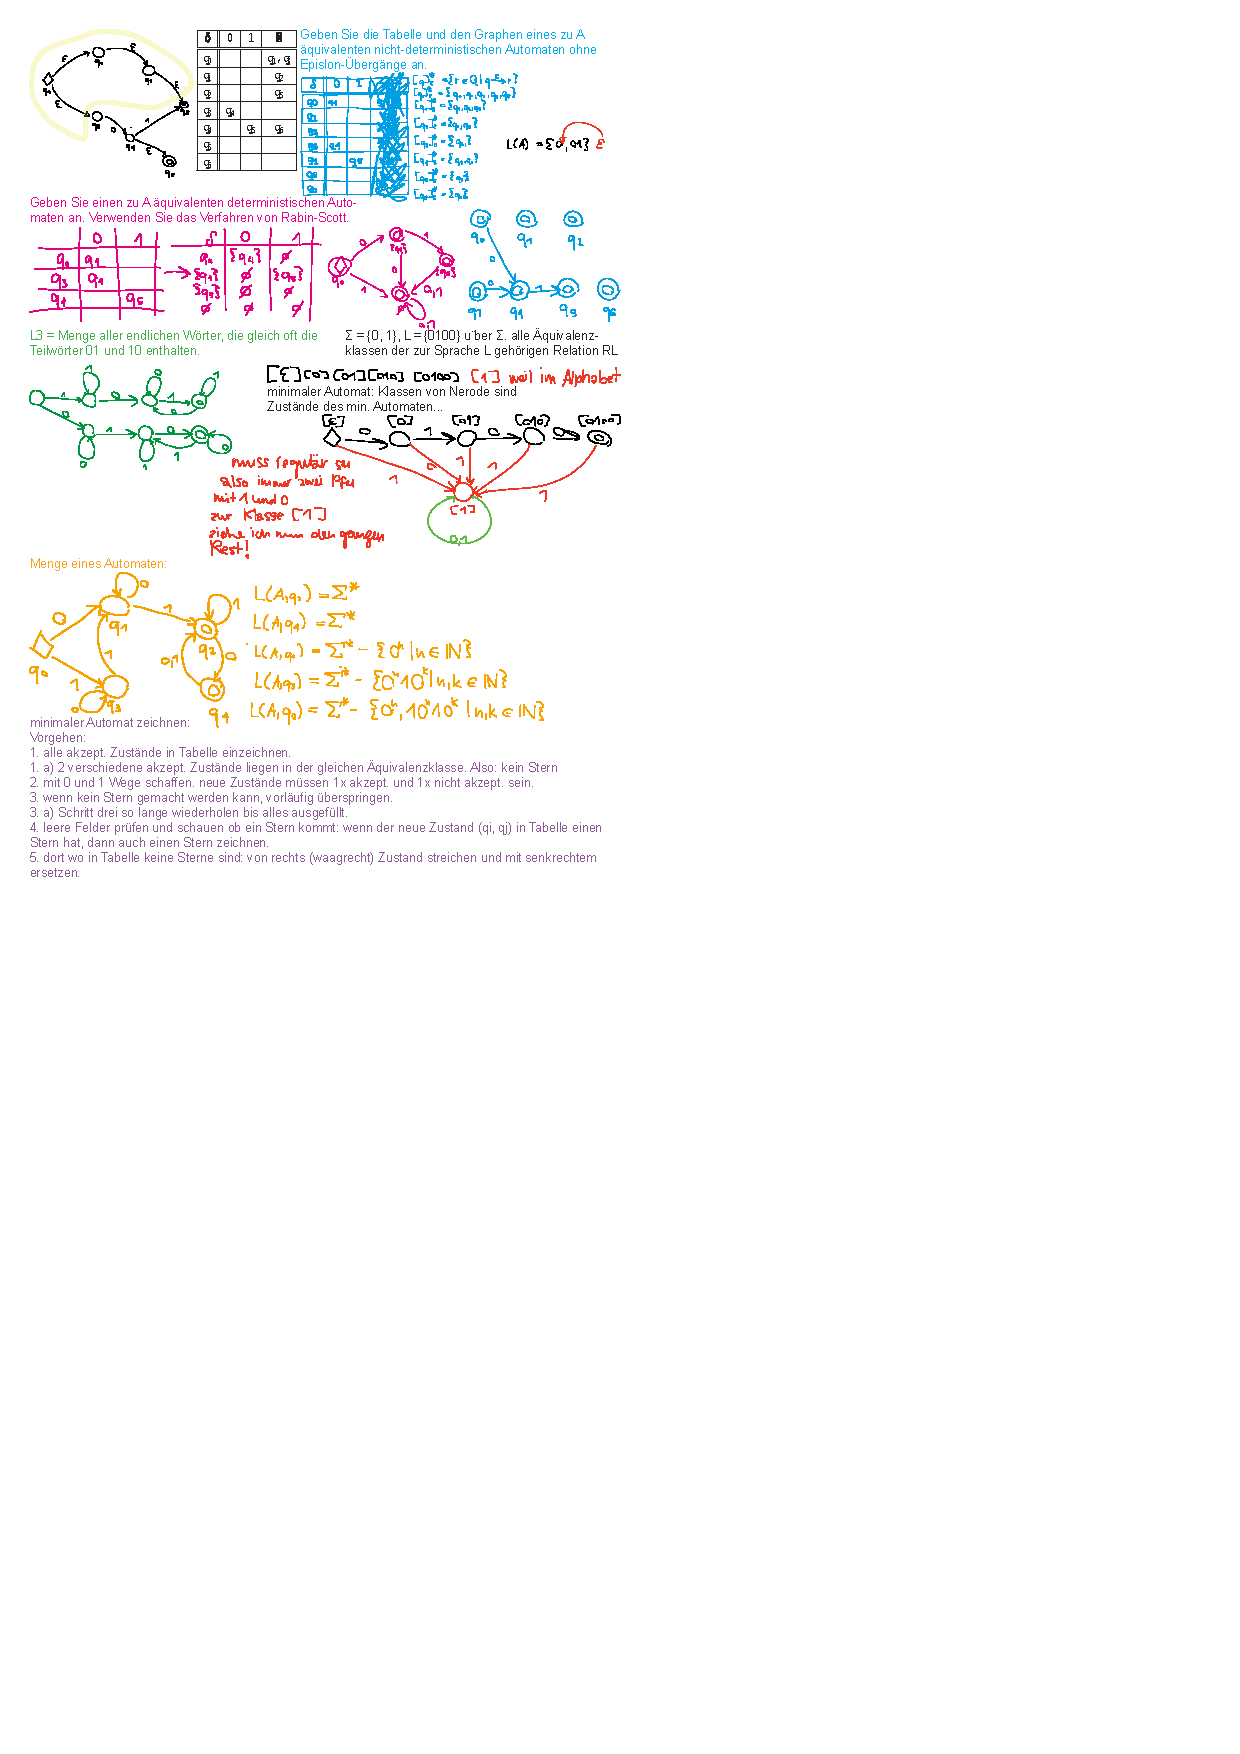
\includegraphics[width=0.45\textwidth,keepaspectratio]{Bild1Zufa.pdf}\\












\end{document}